\chapter{\label{ch:waveletprojection}Wavelet radiosity}
I previous sections projection methods and wavelet has been described. Now we describe the use of wavelet basis for projection method and its advantages. 
We first start with the use of our wavelet basis for expanding our unknown radiosity function B(x) as linear combination of wavelet basis.\\

$B(x) = b_{\phi_0}\phi_0(x)+\sum_{i,j}^{\inf,\inf}b_{\psi_{i,j}}\psi_{i,j}(x)$\\,
where $b_{\phi_0}$ and $b_{\psi_{i,j}}$ coefficients are inner products\\
$b_{\psi_{i,j}}=<B(x),psi_{i,j}(x)>$
From inner product point of view, we find that the small coefficients occur because wavelet functions have vanishing moments.
{\bf define vanishing moments}\\

different wavelet have different vanishing moments. For example Haar wavelet have one vanishing moment. Due to this a function which is nearly constant over the support of wavelet basis function will have coefficient value near 0 corresponding to that wavelet basis function. Similarly linear Legendre multi-wavelets have two vanishing moment, hence function nearly linear will have near 0 coefficient corresponding to that wavelet basis function. This is the advantage of using wavelet basis over box function as basis.\\

Once we project the radiosity function into wavelet basis we need to operate the integral on the projected 

Consider a 2D scene consisting of the two line segment of length 1 meter and at distance of 0.5 meter (see figure (2)). \\

{\bf show figue 2}\\

{\bf explain about the kernel sparsity of wavelet projection }\\


\begin{figure}[tbh]
\centering{}
\captionsetup{justification=centering}
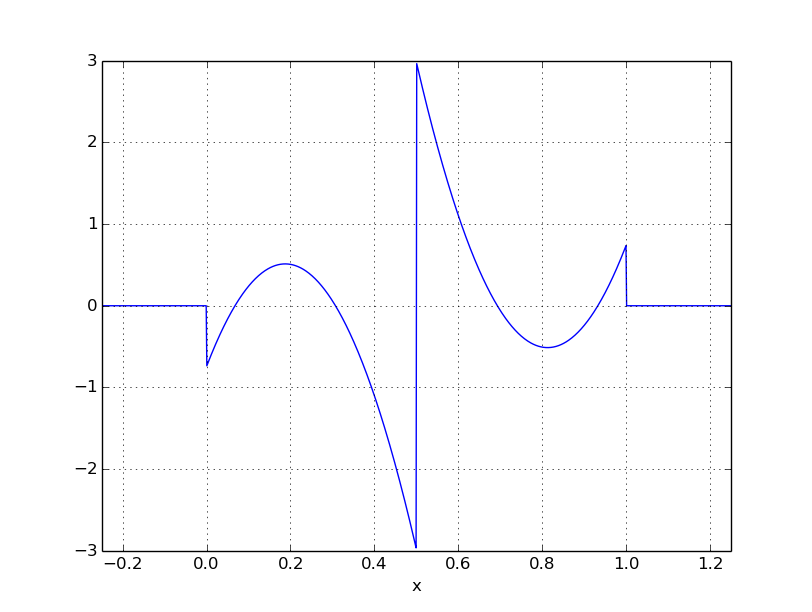
\includegraphics[width=3in]{qlmwpsi2.png}
\caption{\label{fig:replacethis6}flatland1 with $dist=0.25$ kernel sparsity plot haar wavelet}
\end{figure}

\begin{figure}[tbh]
\centering{}
\captionsetup{justification=centering}
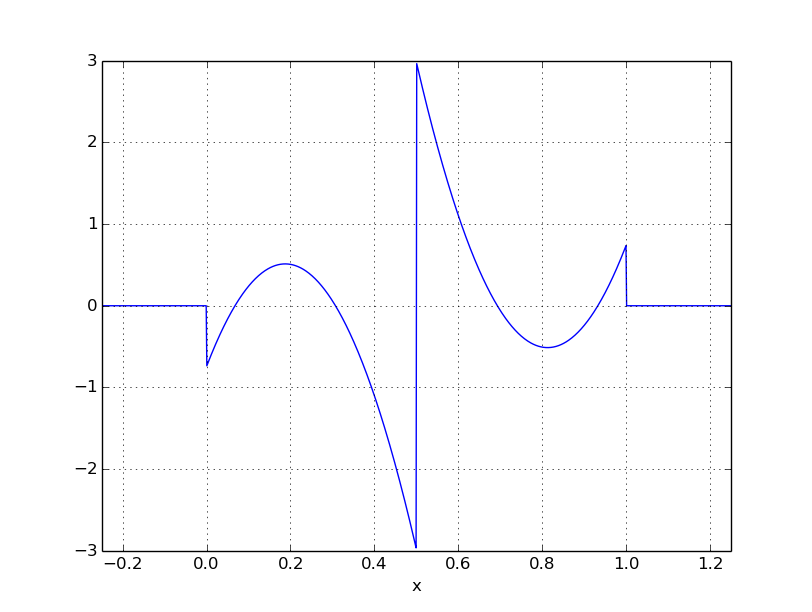
\includegraphics[width=3in]{qlmwpsi2.png}
\caption{\label{fig:replacethis7}flatland1 with $dist=0.25$ kernel sparsity plot llmw wavelet}
\end{figure}

\begin{figure}[tbh]
\centering{}
\captionsetup{justification=centering}
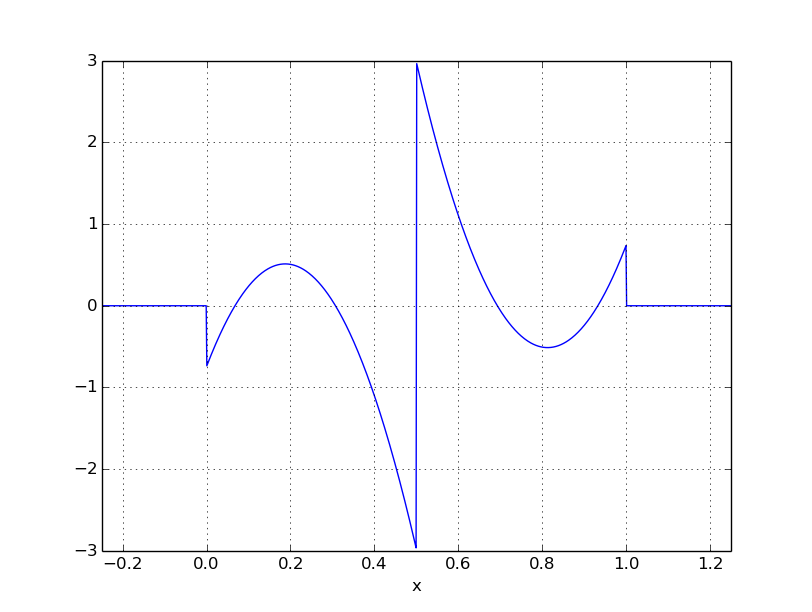
\includegraphics[width=3in]{qlmwpsi2.png}
\caption{\label{fig:replacethis8}flatland1 with $dist=0.25$ kernel sparsity plot qlmw wavelet}
\end{figure}


\begin{figure}[tbh]
\centering{}
\captionsetup{justification=centering}
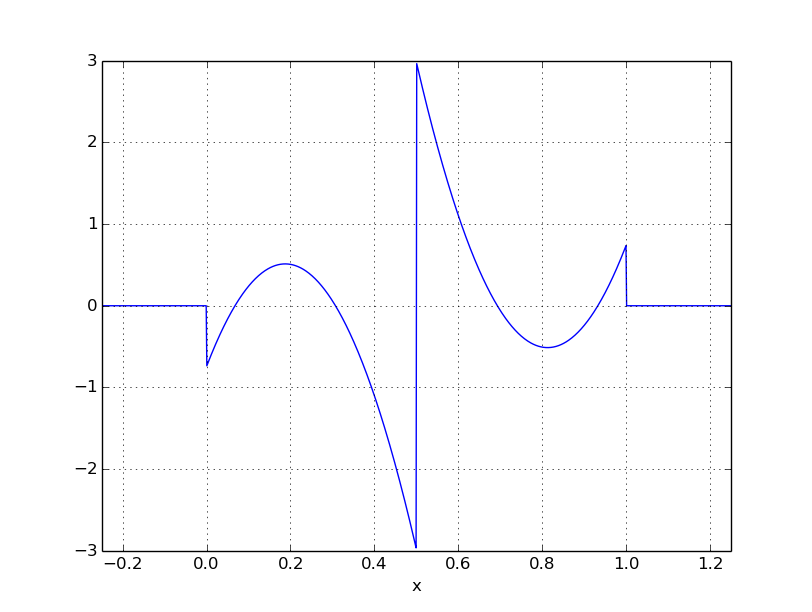
\includegraphics[width=3in]{qlmwpsi2.png}
\caption{\label{fig:replacethis9}flatland2  kernel sparsity plot haar wavelet}
\end{figure}

\begin{figure}[tbh]
\centering{}
\captionsetup{justification=centering}
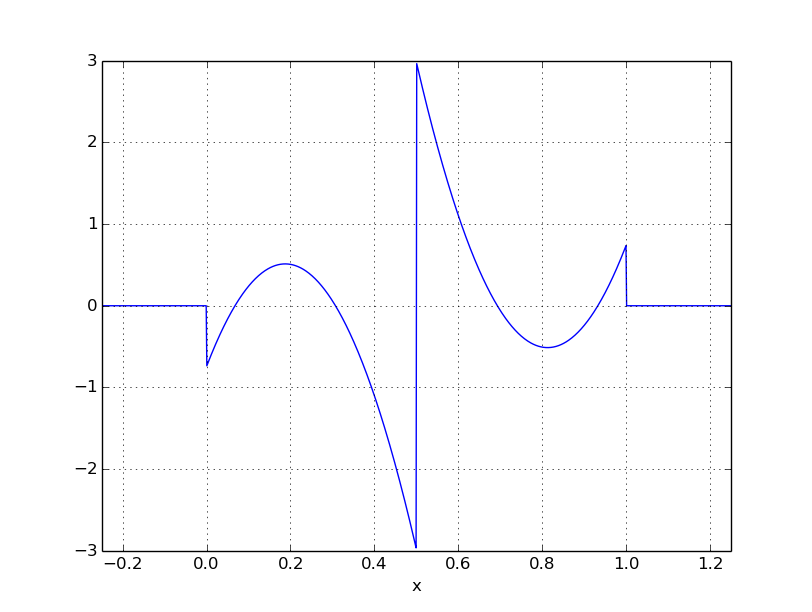
\includegraphics[width=3in]{qlmwpsi2.png}
\caption{\label{fig:replacethis10}flatland2  kernel sparsity plot  llmw wavelet}
\end{figure}

\begin{figure}[tbh]
\centering{}
\captionsetup{justification=centering}
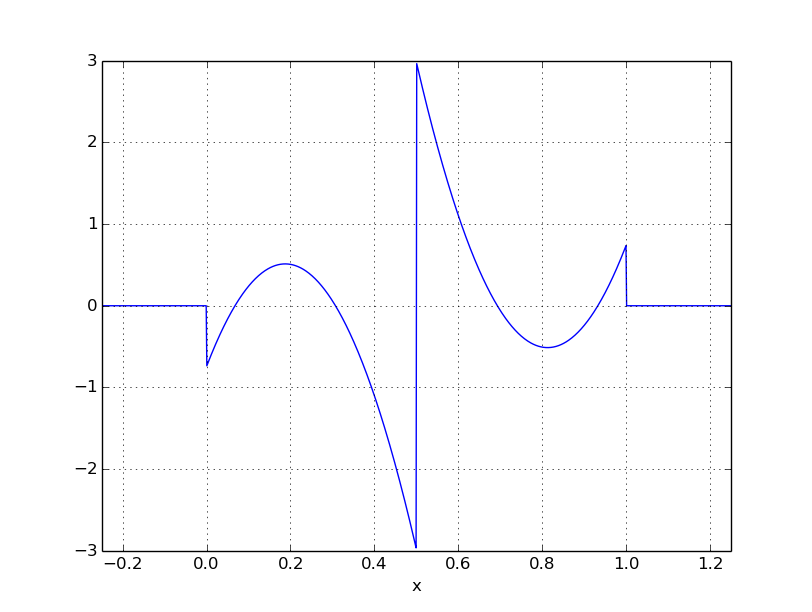
\includegraphics[width=3in]{qlmwpsi2.png}
\caption{\label{fig:replacethis11}flatland2 kernel sparsity plot qlmw wavelet}
\end{figure}

{\bf expalin about 2D and 4d wavelet function (tensor product)}